% -*- mode: LaTeX; TeX-PDF-mode: t; -*- 
% LaTeX path to the root directory of the current project
% from the directory in which this file resides
% and path to econtexPaths which defines the rest of the paths like \FigDir
\providecommand{\econtexRoot}{}\renewcommand{\econtexRoot}{.}
\providecommand{\econtexPaths}{}\renewcommand{\econtexPaths}{econtexPaths}
% -*- mode: LaTeX; TeX-PDF-mode: t; -*- 
% The \commands below are required to allow sharing of the same base code via Github between TeXLive on a local machine and Overleaf (which is a proxy for "a standard distribution of LaTeX").  This is an ugly solution to the requirement that custom LaTeX packages be accessible, and that Overleaf prohibits symbolic links
\providecommand{\packages}{\econtexRoot/Resources/texmf-local/tex/latex}
\providecommand{\econtex}{\packages/econtex}
\providecommand{\econark}{\econtexRoot/Resources/texmf-local/tex/latex/econark}
\providecommand{\econtexSetup}{\econtexRoot/Resources/texmf-local/tex/latex/econtexSetup}
\providecommand{\econarkSetup}{\econtexRoot/Resources/texmf-local/tex/latex/econarkSetup}
\providecommand{\econtexShortcuts}{\econtexRoot/Resources/texmf-local/tex/latex/econtexShortcuts}
\providecommand{\econtexBibMake}{\econtexRoot/Resources/texmf-local/tex/latex/econtexBibMake}
\providecommand{\econtexBibStyle}{\econtexRoot/Resources/texmf-local/bibtex/bst/econtex}
\providecommand{\econtexBib}{economics}
\providecommand{\notes}{\econtexRoot/Resources/texmf-local/tex/latex/handout}
\providecommand{\handoutSetup}{\econtexRoot/Resources/texmf-local/tex/latex/handoutSetup}
\providecommand{\handoutShortcuts}{\econtexRoot/Resources/texmf-local/tex/latex/handoutShortcuts}
\providecommand{\handoutBibMake}{\econtexRoot/Resources/texmf-local/tex/latex/handoutBibMake}
\providecommand{\handoutBibStyle}{\econtexRoot/Resources/texmf-local/bibtex/bst/handout}

\providecommand{\FigDir}{\econtexRoot/Figures}
\providecommand{\CodeDir}{\econtexRoot/Code}
\providecommand{\DataDir}{\econtexRoot/Data}
\providecommand{\SlideDir}{\econtexRoot/Slides}
\providecommand{\TableDir}{\econtexRoot/Tables}
\providecommand{\ApndxDir}{\econtexRoot/Appendices}

\providecommand{\ResourcesDir}{\econtexRoot/Resources}
\providecommand{\rootFromOut}{..} % APFach back to root directory from output-directory
\providecommand{\LaTeXGenerated}{\econtexRoot/LaTeX} % Put generated files in subdirectory
\providecommand{\econtexPaths}{\econtexRoot/Resources/econtexPaths}
\providecommand{\LaTeXInputs}{\econtexRoot/Resources/LaTeXInputs}
\providecommand{\LtxDir}{LaTeX/}
\providecommand{\EqDir}{\econtexRoot/Equations} % Put generated files in subdirectory

\providecommand{\titlepagecustom}{\LaTeXInputs/titlepagecustom}


\documentclass[\econtexRoot/HAFiscal]{subfiles}
\onlyinsubfile{\externaldocument{\econtexRoot/HAFiscal}} % Get xrefs -- esp to apndx -- from main file; only works if main file has already been compiled

\begin{document}
	
\FloatBarrier
\hypertarget{hank}{}\par\section{Robustness in a HANK and SAM Model}
\notinsubfile{\label{sec:hank}}


The main results of this paper are presented in a partial equilibrium setup with aggregate demand effects that do not arise from general equilibrium effects. We think there are many advantages to studying the welfare and multiplier effects in this setting without embedding the model in general equilibrium.  First, general equilibrium models often struggle to adequately capture the feedback mechanisms between consumption and income, particularly the asymmetric nature of these relationships during recessionary versus expansionary periods. Additionally, a complete general equilibrium treatment would necessitate the analysis of numerous complex channels including investment dynamics, firm ownership structures and dividend distribution policies, inventory management, and international trade flows—elements that, while important in their own right, would potentially obscure the core mechanisms we aim to investigate.

Despite the advantages of our partial equilibrium approach, here we complement our analysis with a general equilibrium HANK and SAM model, as standard as possible, that is able to capture supply-side effects that are absent from the partial equilibrium model. In particular, fiscal policies can generate labor market responses that our partial equilibrium analysis does not address. These supply-side channels can affect both the welfare implications and the fiscal multipliers of different policy interventions. Furthermore, standard to the HANK and SAM literature, the general equilibrium model generates a self-reinforcing precautionary saving channel that amplifies business cycles. During a recession, heightened unemployment risk prompts households to increase savings and reduce consumption which in turn weakens both aggregate and labor demand. The resulting decline in labor demand further raises unemployment risk, reinforcing precautionary savings.

We embed the consumption choices of our households—--with heterogeneity over education type and discount factors—--in a New Keynesian model with search and matching frictions that closely follows \cite{Du2024}, which, in turn, is in spirit of the seminal work of \cite{Ravn2017}. Aside from the consumption block of the model, the framework is standard and follows from the HANK and SAM literature. The model features nominal price rigidities \`{a} la Rotemberg, a monetary authority that sets the nominal interest rate following a standard Taylor rule that responds to inflation, and a fiscal authority that taxes labor income and borrows debt from households to fund unemployment insurance and interest on past debt. As in \cite{Gornemann2021}, \cite{Bardoczy2022}, and \cite{gravesUnemployment}, households randomly search for jobs and match with a labor agency that sells labor to intermediate good producers. Complete details of the model are provided in appendix \ref{sec:hank_appendix}. 

The general equilibrium structure generates fiscal multipliers through an intertemporal Keynesian cross mechanism, which becomes particularly pronounced when monetary policy is passive. Moreover, the search and matching framework allows the employment rate to respond to policy interventions, allowing us to capture both demand and supply effects of fiscal policies.

Our approach in this section relies on linearizing the macro dynamics of the model and employs the Sequence Space Jacobian methods developed by \cite{Auclert2021}. This linearization imposes certain constraints on our analysis. Notably, we cannot evaluate the effects of different policies starting from a deep recessionary state, as we do in our main results.\footnote{One approach to overcome this limitation, which could be used in future work, is described in \cite{bmpMITshocks}.} This limitation prevents us from conducting welfare comparisons between recessionary periods and the steady state. Additionally, the Keynesian cross mechanism embedded in the model exhibits uniform behavior regardless of the degree of economic slack—--a feature that stands in contrast to the state-dependent multipliers we apply in our partial equilibrium analysis.\footnote{We note two additional technical limitations of our general equilibrium implementation. First, stimulus payments in the model are specified as proportional to permanent income, rather than as means-tested fixed dollar amounts as implemented in practice and in our partial equilibrium framework. Second, splurge behavior only occurs out of equilibrium.} 



The consumption response in this general equilibrium model to each of the three policies is shown in the top row of Figure~\ref{fig:HANK_IRFs}. For each of the three fiscal policies, we have shown the consumption response under three different monetary policy rules: 1) an active Taylor rule with a coefficient of 1.5 on inflation; 2) a fixed nominal rate (simulating an effective lower bound); and 3) a fixed real rate (closest in spirit to our partial equilibrium analysis).

%Old figure with just the impulse response
\begin{comment}
\begin{figure}[th]
	\begin{center}
		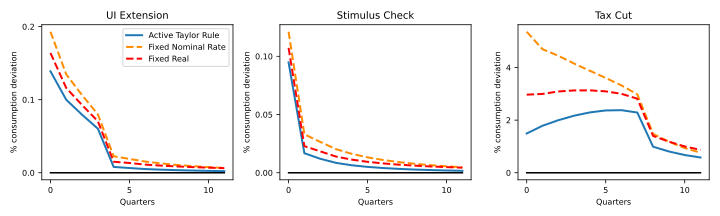
\includegraphics[width=.9\textwidth]{../Figures/HANK_IRFs_w_splurge}
		\caption{Consumption Impulse Responses to Each Policy in the HANK and SAM Model}
		\notinsubfile{\label{fig:HANK_IRFs}}
	\end{center}
\end{figure}
\end{comment}


\begin{figure}[htb]
	\centering
	\begin{subfigure}[b]{.33\linewidth}
		\centering
		\includegraphics[width=\linewidth]{\econtexRoot/Code/HA-Models/FromPandemicCode/Figures/HANK_transfer_irf}
		\caption{stimulus check - IRF}
		\notinsubfile{\label{fig:hank_stimulus_irf}}
	\end{subfigure}%
	\begin{subfigure}[b]{.33\linewidth}
		\centering
		\includegraphics[width=\linewidth]{Code/HA-Models/FromPandemicCode/Figures/HANK_UI_irf}
		\caption{UI extension - IRF}
		\notinsubfile{\label{fig:hank_UI_irf}}
	\end{subfigure}%
	\begin{subfigure}[b]{.33\linewidth}
		\centering
		\includegraphics[width=\linewidth]{Code/HA-Models/FromPandemicCode/Figures/HANK_tax_irf}
		\caption{payroll tax cut - IRF}
		\notinsubfile{\label{fig:hank_tax_irf}}
	\end{subfigure}\\
	\begin{subfigure}[b]{.33\linewidth}
		\centering
		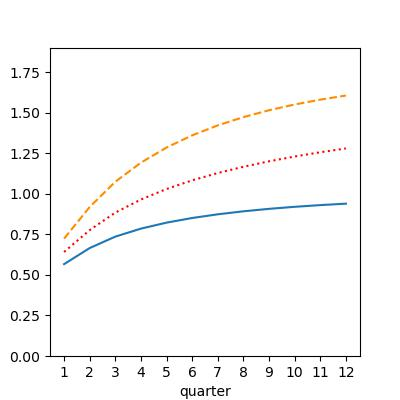
\includegraphics[width=\linewidth]{\econtexRoot/Code/HA-Models/FromPandemicCode/Figures/HANK_transfer_multiplier}
		\caption{stimulus check - cumulative multiplier}
		\notinsubfile{\label{fig:HANK_transfer_multiplier}}
	\end{subfigure}%
	\begin{subfigure}[b]{.33\linewidth}
		\centering
		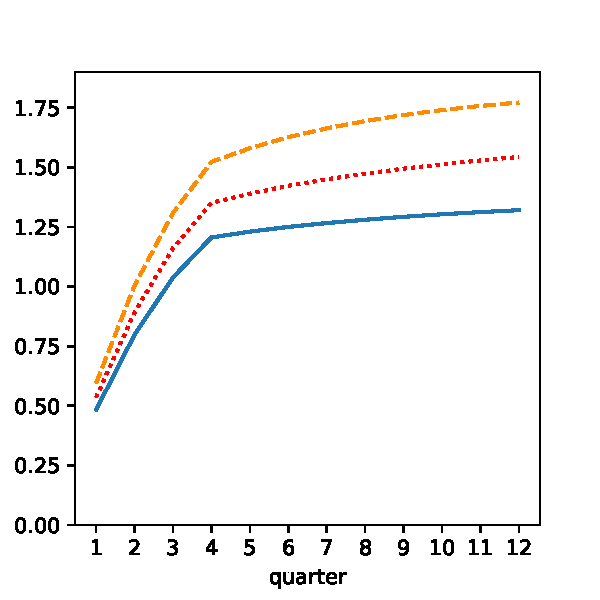
\includegraphics[width=\linewidth]{Code/HA-Models/FromPandemicCode/Figures/HANK_UI_multiplier}
		\caption{UI extension - cumulative multiplier}
		\notinsubfile{\label{fig:HANK_UI_multiplier}}
	\end{subfigure}%
	\begin{subfigure}[b]{.33\linewidth}
		\centering
		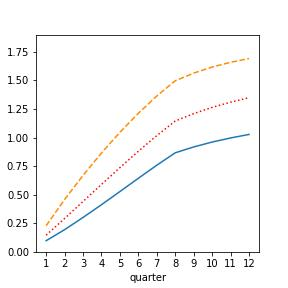
\includegraphics[width=\linewidth]{Code/HA-Models/FromPandemicCode/Figures/HANK_tax_multiplier}
		\caption{payroll tax cut - cumulative multiplier}
		\notinsubfile{\label{fig:HANK_tax_multiplier}}
	\end{subfigure}
	\caption{Impulse responses of aggregate consumption to policy shocks as well as cumulative multipliers as a function of the horizon for the three policies.
{\label{fig:HANK_IRFs}}}
\end{figure}



Overall, the IRFs from this model are similar to those from the partial equilibrium analysis, especially under the fixed real-rate rule.
Note that the magnitude of the consumption response to the UI extension is lower than in our main analysis---a consequence of lower long-term unemployment in this HANK exercise of deviating from the steady state.\footnote{By contrast, our main analysis considers deviations from a recessionary scenario.
Note that the dynamics of the UI extension IRF are also somewhat faster acting.
This is because, under the recession that we study in the partial equilibrium analysis, the large mass of newly-unemployed households do not start receiving extended UI for six months.
} Furthermore, although we are unable to repeat our welfare analysis under a recession in this model, the distributional effects of the policies are similar.
Most importantly, the mechanism leading to far greater welfare benefits for the UI extension, namely that the newly unemployed have high marginal utility, are robust to the supply-side effects of a general equilibrium HANK and SAM model.

\begin{figure}[th]
	\begin{center}
		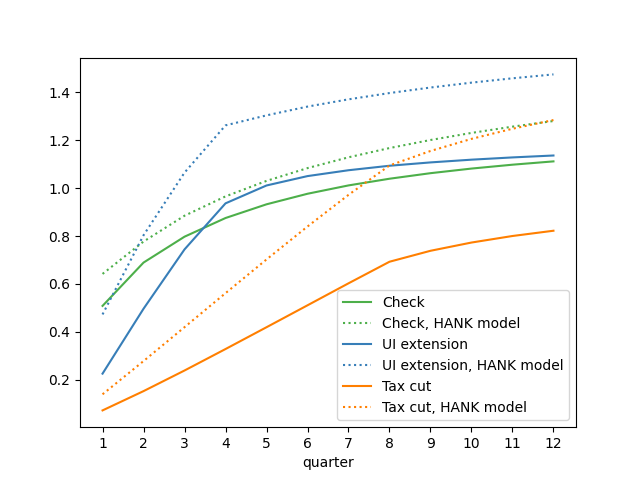
\includegraphics[width=.9\textwidth]{\econtexRoot/Code/HA-Models/FromPandemicCode/Figures/Cummulative_multipliers_withHank}
		\caption{Consumption multiplier as a function of the horizon for the three policies in the partial equilibrium vs the HANK model}
		\parbox{16cm}{\small \vspace{.15cm} \textbf{Note}: In the partial equilibrium model, policies are implemented during a recession with aggregate demand effect active.\normalsize}
		\notinsubfile{\label{fig:HANK_multipliers}}
	\end{center}
\end{figure}


The bottom row of Figure~\ref{fig:HANK_IRFs} shows the corresponding cumulative multipliers for each policy and monetary policy rule.
Figure \ref{fig:HANK_multipliers} compares these consumption multipliers over different horizons under a fixed real rate rule to those in our baseline partial equilibrium model.
The multipliers are bigger in the HANK and SAM model.
Nevertheless, in both models, the relative ranking of the consumption multipliers over time horizons are similar, with the effect of the tax cut substantially smaller than the stimulus check or UI extension policies, despite the inclusion of supply-side effects in this HANK model.
However, in contrast to the partial equilibrium model, towards the end of the period shown the tax cut consumption multiplier is near that of the stimulus check.
This is because the aggregate demand effects in our partial equilibrium model do not continue beyond the recession, dampening the benefits of the tax cut policy---in which much of the extra spending occurs after the recession is over---relative to the stimulus check and extended UI policies.


\ifthenelse{\boolean{Web}}{}{
\end{document} \endinput
}
